
\documentclass[11pt]{exam} % https://www.ctan.org/pkg/exam?lang=en

\usepackage[lmargin=1.in,rmargin=1.in,tmargin=1.in,bmargin=1in]{geometry}
\usepackage{setspace}
\usepackage[pdftex]{graphicx}
\usepackage{titling}
\usepackage[
	pdfauthor={Brian Weinstein},
	pdftitle={Homework 1},
	bookmarks=true,
	colorlinks=true,
	linkcolor=blue,
	urlcolor=blue,
	citecolor=blue,
	pdftex,
	linktocpage=true
	]{hyperref}
\usepackage[textsize=tiny]{todonotes}
\usepackage{float}
\setlength\parindent{0pt}
\usepackage{lipsum}
\usepackage{amsmath}
\usepackage{caption}


\qformat{\textbf{Problem \thequestion: \thequestiontitle}\quad \hfill}


\pagestyle{headandfoot}
\runningheadrule
\firstpageheader{}{}{}
\runningheader{\theauthor}{\thetitle}{\thedate}
\firstpagefooter{}{\thepage}{}
\runningfooter{}{\thepage}{}


\usepackage{xcolor}
\usepackage{adjustbox}
\usepackage{verbatim}
\definecolor{shadecolor}{rgb}{.9, .9, .9}

\newenvironment{code}%
   {\par\noindent\adjustbox{margin=1ex,bgcolor=shadecolor,margin=0ex \medskipamount}\bgroup\minipage\linewidth\verbatim}%
   {\endverbatim\endminipage\egroup}

\newenvironment{codeSmall}%
   {\par\noindent\adjustbox{margin=1ex,bgcolor=shadecolor,margin=0ex \medskipamount}\bgroup\minipage\linewidth\verbatim\footnotesize}%
   {\endverbatim\endminipage\egroup}

\newcommand{\ramsey}{\href{http://www.statisticalsleuth.com/}{Ramsey }}



\begin{document}


\title{STAT W4201 001, Homework 8}
\author{Brian Weinstein (bmw2148)}
\date{Apr 6, 2016}
\maketitle

Code is attached here and also posted at \href{https://github.com/BrianWeinstein/advanced-data-analysis}{https://github.com/BrianWeinstein/advanced-data-analysis}. Where relevant, code snippets and output are are included in-line.

\begin{questions}


\titledquestion{\ramsey 12.17}
\setlength{\parindent}{1em}


\textit{It is desired to determine whether the pollution variables (13, 14, and 15) are associated with mortality, after the other climate and socioeconomic variables are accounted for. (Note: These data have problems with influential observations and with lack of independence due to spatial correlation; these problems are ignored for purposes of this exercise.)}

\begin{parts}
\setlength{\parindent}{1em}


\part \textit{With mortality as the response, use a Cp plot and the BIC to select a good-fitting regression model involving weather and socioeconomic variables as explanatory. To the model with the lowest Cp, add the three pollution variables (transformed to their logarithms) and obtain the p-value from the extra-sum-of-squares F-test due to their addition.}

A matrix of pairwise scatterplots is shown in Figure \ref{fig:1a_pairs}.

\begin{figure}[!h]
	\centering
	\captionsetup{width=0.8\textwidth}
	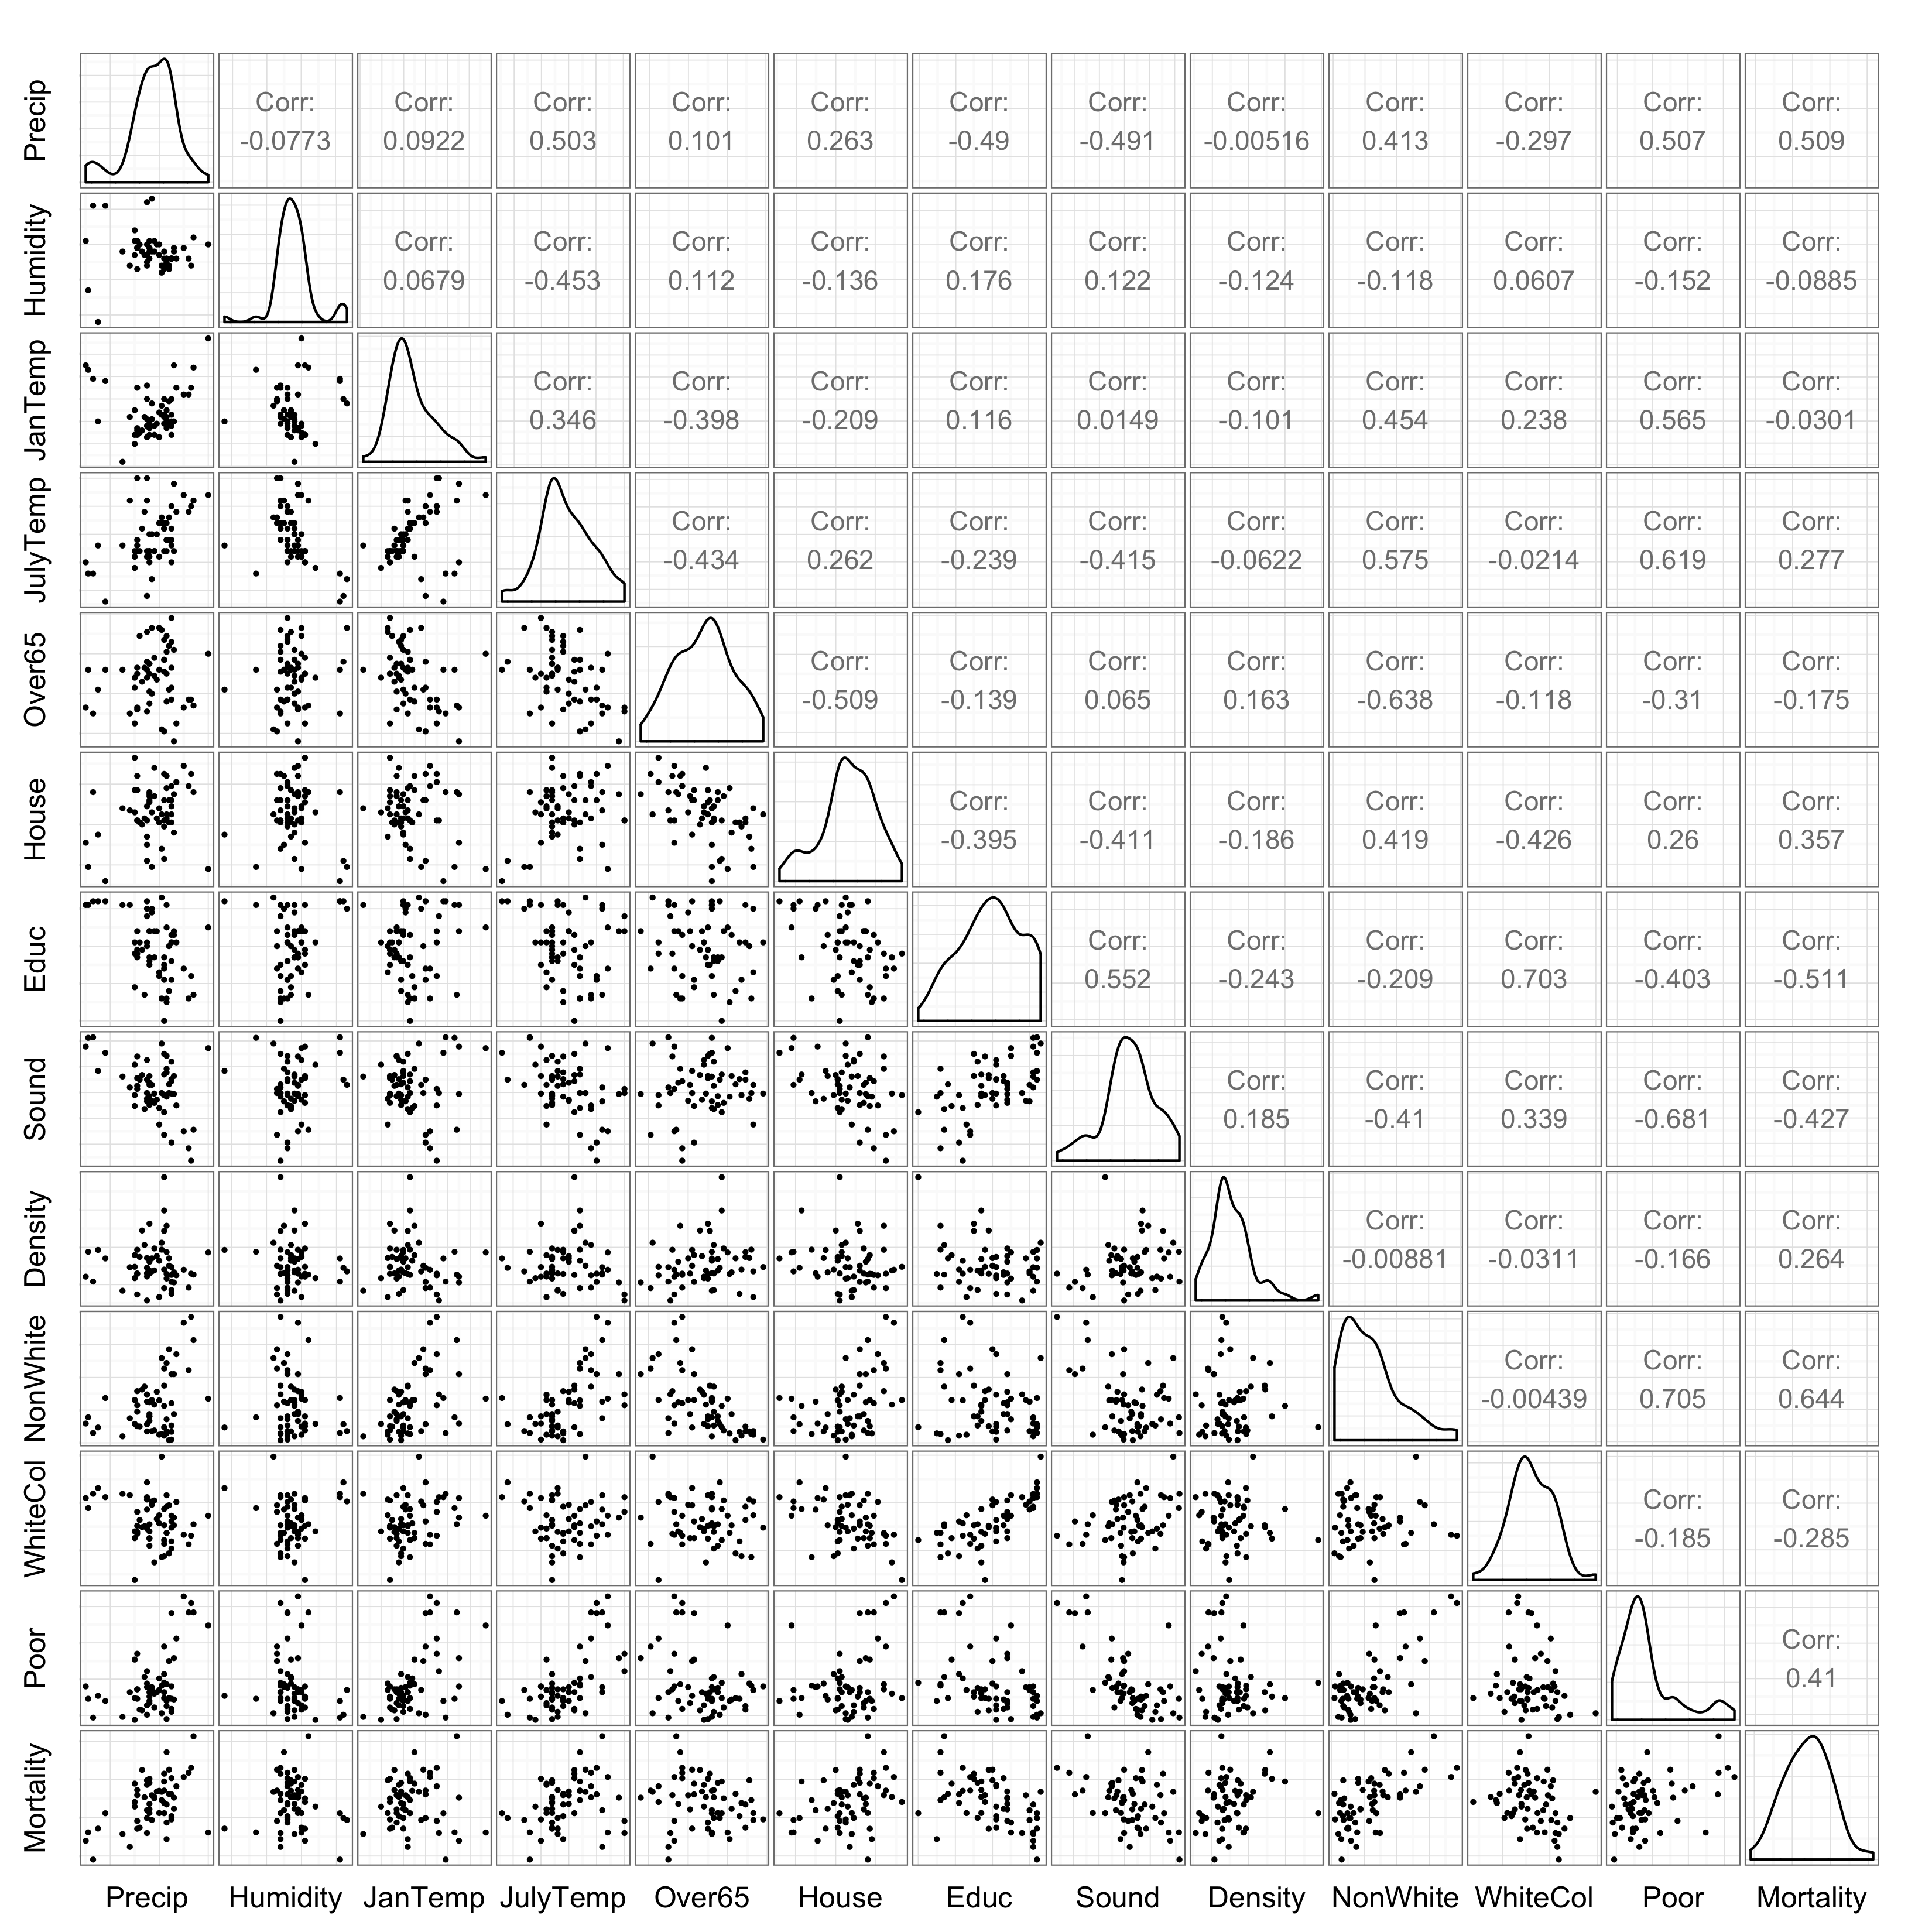
\includegraphics[width=\textwidth]{1a_pairs.png}
	\caption{Pairwise scatterplots of the weather and socioeconomic variables from the ``Pollution and Mortality'' dataset.}
	\label{fig:1a_pairs}
\end{figure}

Initial investigation of the pairwise scatterplots indicate a couple of things.
\begin{itemize}

\item The effect of the JanTemp, JulyTemp, Over65, and House variables on Mortality are all nonlinear. As each of these variables increases (marginally, at least), Mortality first increases and then decreases. Adding quadratic terms for each of these variables will help model this behavior.

\item Many of the explanatory variables are highly correlated (e.g., JanTemp and JulyTemp, Educ and Sound, Humidity and WhiteCol, etc.). The inclusion of all of these variables will likely be unnecessary in the final model, but we keep them here so that it's unlikely we miss an important relationship during initial investigation.

\end{itemize}

Using the \textit{leaps::regsubsets} R function, we first do an exhaustive search over all $2^16$ possible models (using the original 12 weather and socioeconomic variables, and the 4 squared terms), recording the Cp and BIC for the best few models of each size. We then ignore the models that include a squared variable but don't include the associated linear variable (as per section 12.6).

A Cp plot is shown in Figure \ref{fig:1a_cp} for the remaining models. To reduce clutter, I've only included those models with relatively low Cp statistics.

\begin{figure}[!h]
	\centering
	\captionsetup{width=0.8\textwidth}
	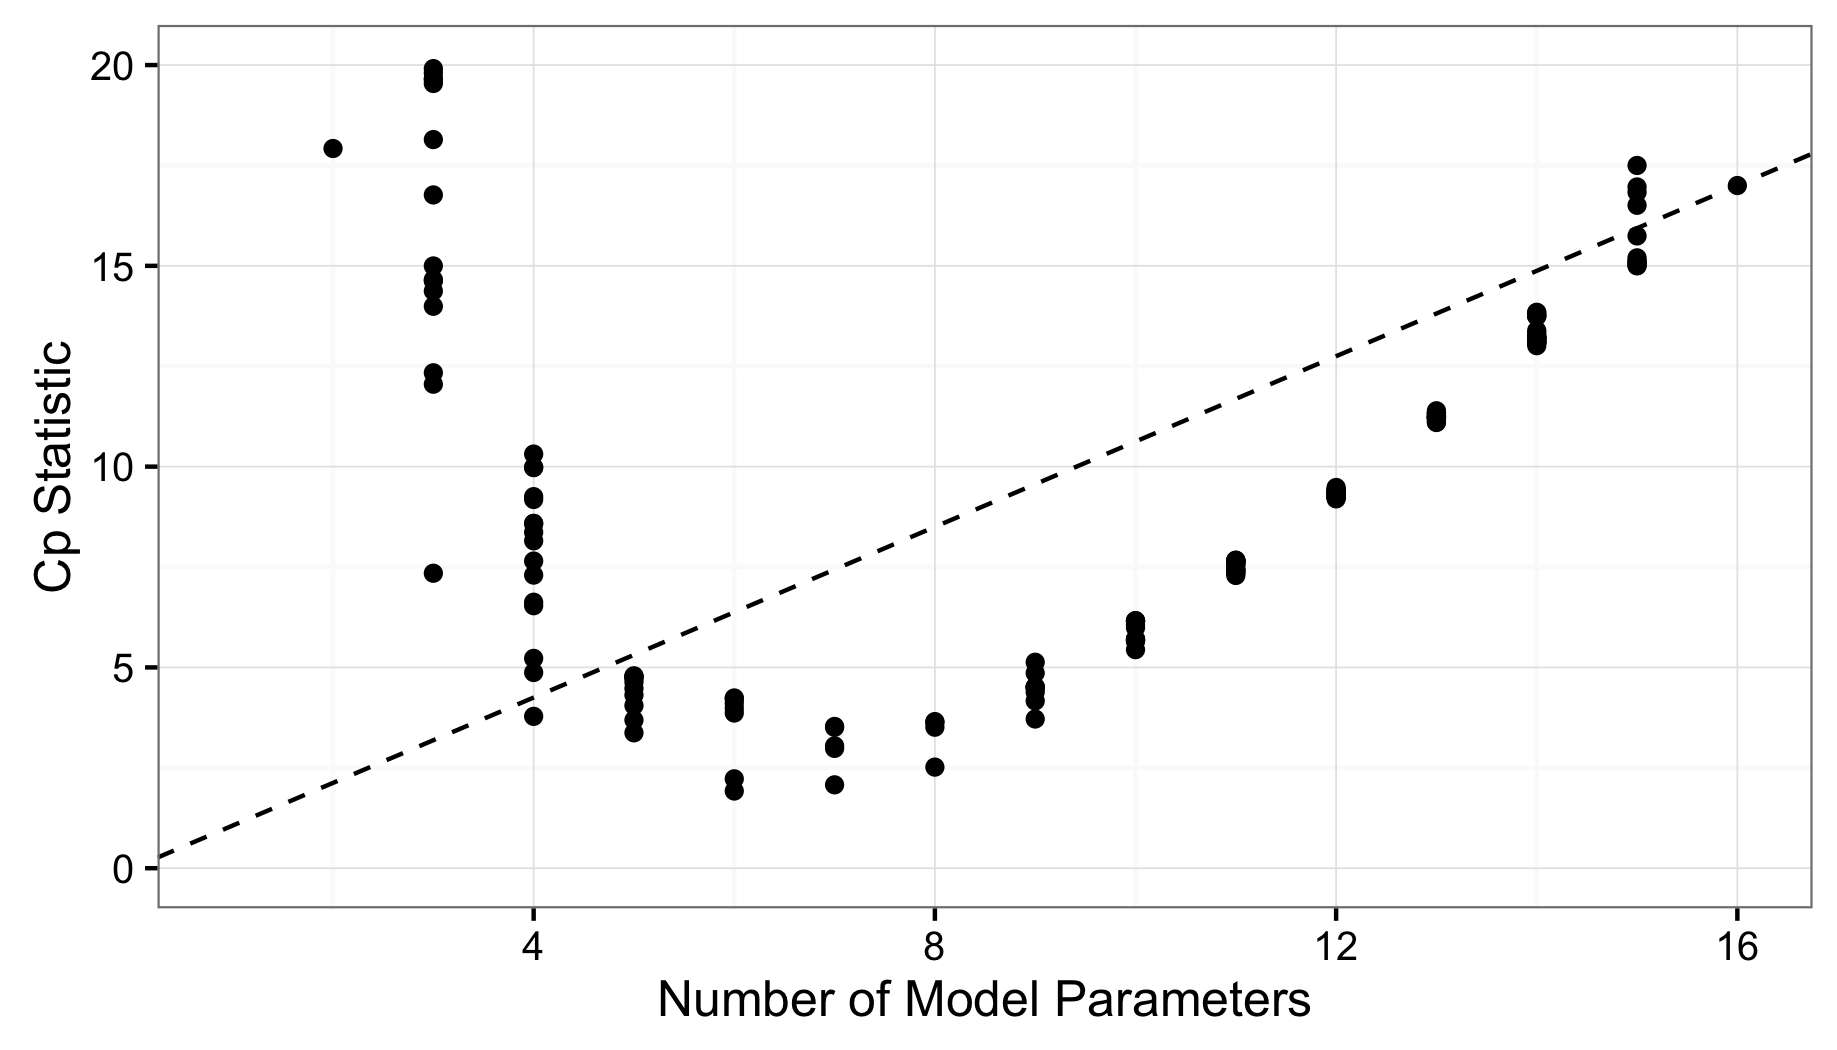
\includegraphics[width=4.25in]{1a_cp.png}
	\caption{Cp plot for the ''good subset models`` with relatively low Cp statistics.}
	\label{fig:1a_cp}
\end{figure}

The model with the lowest Cp statistic is the one that includes Precip, JanTemp, JulyTemp, Educ, Density, and NonWhite, plus an intercept term. For this model, the Cp statistic is $1.922$. This model has the 3rd lowest BIC, and we continue with this set of variables for the remainder of the problem.

To the 6-variable model, we add the log-transformed pollution variables and perform an extra-sum-of-squares F-test as shown below.

\begin{codeSmall}
> anova(lmBestSubsetPoll, lmBestSubset)
Analysis of Variance Table

Model 1: Mortality ~ Precip + JanTemp + JulyTemp + Educ + Density + NonWhite + 
    log(HC) + log(NOX) + log(SO2)
Model 2: Mortality ~ Precip + JanTemp + JulyTemp + Educ + Density + NonWhite
  Res.Df   RSS Df Sum of Sq     F   Pr(>F)   
1     50 52712                               
2     53 66518 -3    -13806 4.365 0.008313 **
---
Signif. codes:  0 ‘***’ 0.001 ‘**’ 0.01 ‘*’ 0.05 ‘.’ 0.1 ‘ ’ 1
\end{codeSmall}

Using the results from the 6-variable model and the 9-variable model (including the 6 variables, plus the 3 pollution variables), the data provides convincing evidence that the three pollution variables are associated with mortality (p-value = 0.008313; extra sum of squares F-test).


\part \textit{Repeat part (a) but use a sequential variable selection technique (forward selection, backward elimination, or stepwise regression). How does the p-value compare?}

Using forward selection, we select a model that includes NonWhite, Educ, JanTemp, House, JulyTemp, Precip, and Density, plus an intercept term.

To this 7-variable model, we add the log-transformed pollution variables and perform an extra-sum-of-squares F-test as shown below.

\begin{codeSmall}
> anova(lmForwardSubsetPoll, lmForwardSubset)
Analysis of Variance Table

Model 1: Mortality ~ NonWhite + Educ + JanTemp + House + JulyTemp + Precip + 
    Density + log(HC) + log(NOX) + log(SO2)
Model 2: Mortality ~ NonWhite + Educ + JanTemp + House + JulyTemp + Precip + 
    Density
  Res.Df   RSS Df Sum of Sq      F   Pr(>F)   
1     49 50403                                
2     52 63955 -3    -13552 4.3915 0.008162 **
---
Signif. codes:  0 ‘***’ 0.001 ‘**’ 0.01 ‘*’ 0.05 ‘.’ 0.1 ‘ ’ 1
\end{codeSmall}

Using the results from the 7-variable model and the 10-variable model (including the 7 variables, plus the 3 pollution variables), the data provides convincing evidence that the three pollution variables are associated with mortality (p-value = 0.008162; extra sum of squares F-test). Using forward selection, the p-value is almost identical to (just negligibly smaller than) the one found using the model in part (a).

\end{parts}




\titledquestion{\ramsey 12.20}
\setlength{\parindent}{1em}

\textit{The number of species on an island is known to be related to the island's area. Of interest is what other variables are also related to the number of species, after island area is accounted for, and whether the answer differs for native species and nonnative species.}

We first define the ``Nonnative'' species value as the total number of species (Total), minus the number of native species (Native). An initial matrix of pairwise scatterplots indicates both (1) severe outliers, and (2) nonlinear behavior between the explanatory variables and Native and Nonnative.

Testing various variable transformations to reduce outliers and make the data more linear, we find that a good set of explanatory variables is log(Area), log(Elev), log(DistNear), log(1 + DistSc), and log(AreaNear). A matrix of pairwise scatterplots with this set of transformed variables is shown in Figure \ref{fig:2_pairs_tranf}. On the untransformed scale, Isabela island has an Area much larger than the rest of the dataset, but on the log scale this is no longer an issue (for neither the Area variable nor the AreaNear variable).

\begin{figure}[!h]
	\centering
	\captionsetup{width=0.8\textwidth}
	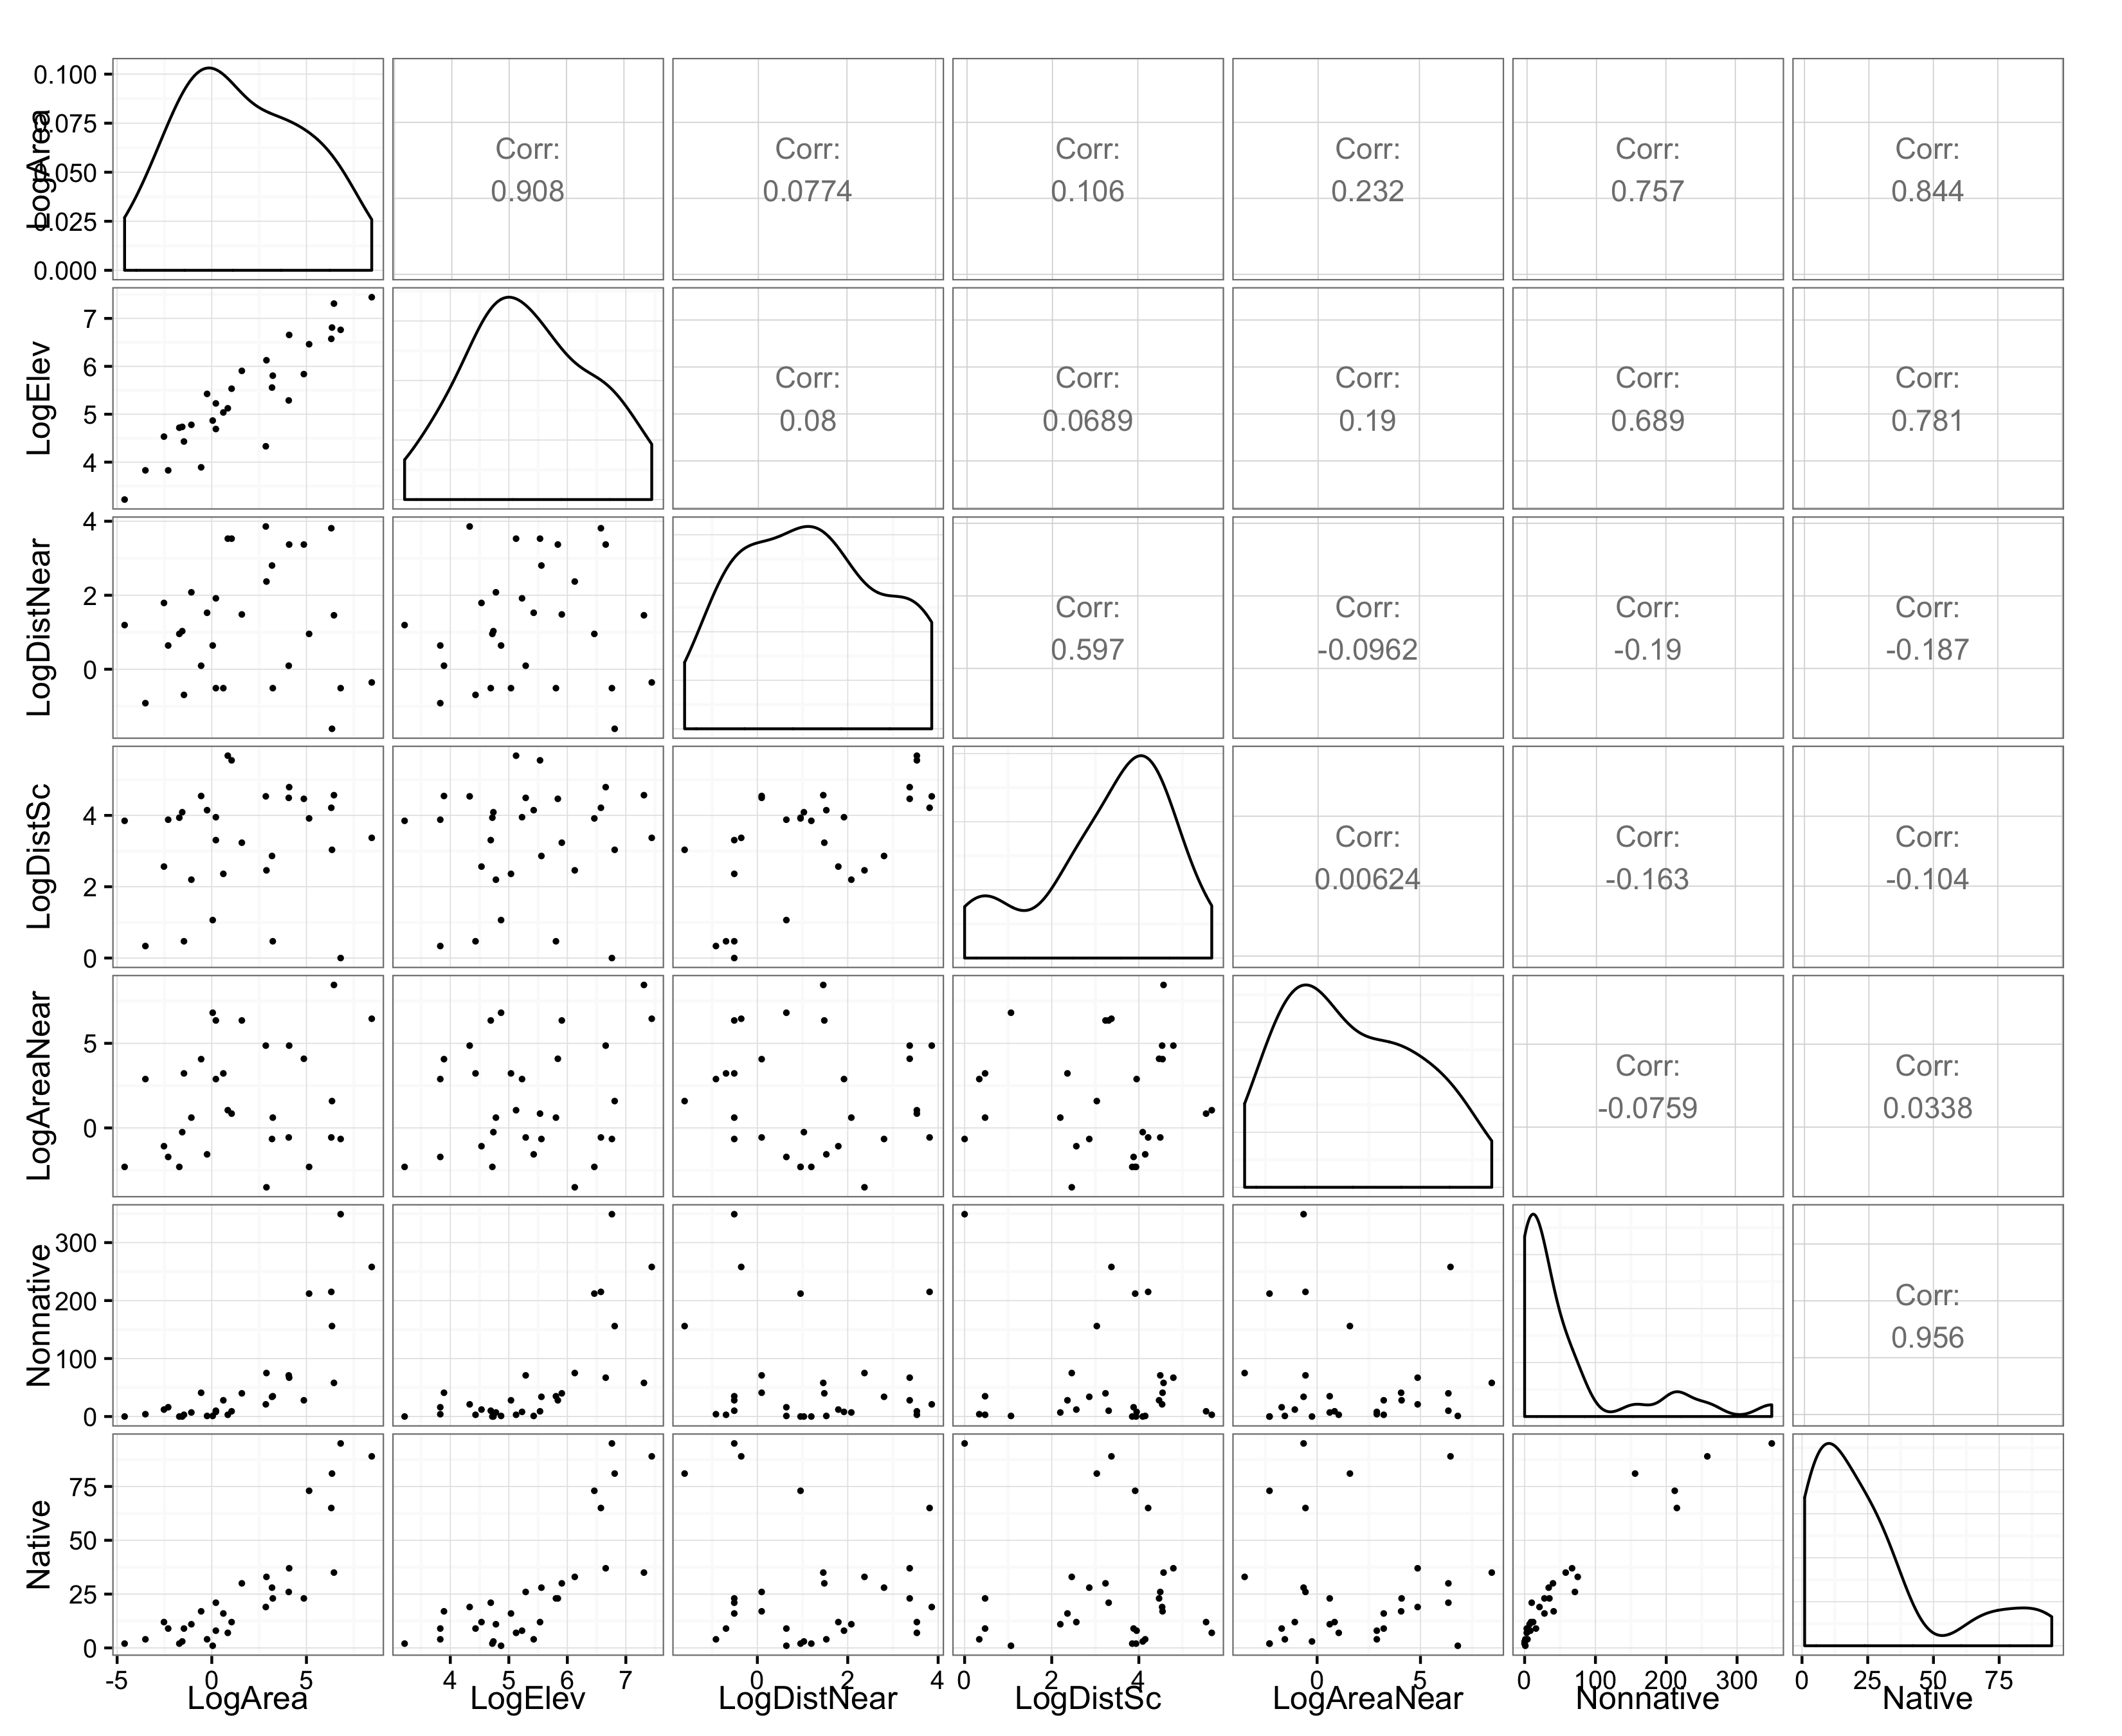
\includegraphics[width=\textwidth]{2_pairs_tranf.png}
	\caption{Pairwise scatterplots of the transformed variables in the ``Galapagos Islands'' dataset.}
	\label{fig:2_pairs_tranf}
\end{figure}


\begin{parts}
\setlength{\parindent}{1em}

\part \textit{Native Species}

A multiple regression of Native on LogArea, LogElev, LogDistNear, LogDistSc, and LogAreaNear is shown below.

\begin{codeSmall}
> # create a linear model with response=Native
> lmNative <- lm(formula = Native ~ LogArea + LogElev +
+                  LogDistNear + LogDistSc + LogAreaNear,
+                data = galapDataTransf)
> summary(lmNative)$coefficients
              Estimate Std. Error    t value     Pr(>|t|)
(Intercept) 17.4186072 26.6342475  0.6539928 0.5193343862
LogArea      6.7877699  1.6800966  4.0401069 0.0004761012
LogElev      1.6306771  5.2281734  0.3119019 0.7578086491
LogDistNear -4.2190775  1.8650490 -2.2621805 0.0330196612
LogDistSc   -0.8665726  1.9225987 -0.4507298 0.6562300815
LogAreaNear -1.6606874  0.7468994 -2.2234419 0.0358553724
\end{codeSmall}$

After accounting for the relationship between Native and Area (where we use the log-transformed value of Area, here), there is suggestive (but inconclusive) evidence that the distance to the nearest island (LogDistNear) is associated with the number of native species on the given island (two sided p-value = 0.0759 for a test that the LogDistNear coefficient is zero). There is moderate evidence that the area of the nearest island (LogAreaNear) is associated with the number of native species on the given island (two sided p-value = 0.0359 for a test that the LogAreaNear coefficient is zero). None of the other variables have a significant relationship with the number of native species.

Examining Cook's Distances for this model in Figure \ref{fig:2a_cd}, none of the observations are influential.

\begin{figure}[!h]
	\centering
	\captionsetup{width=0.8\textwidth}
	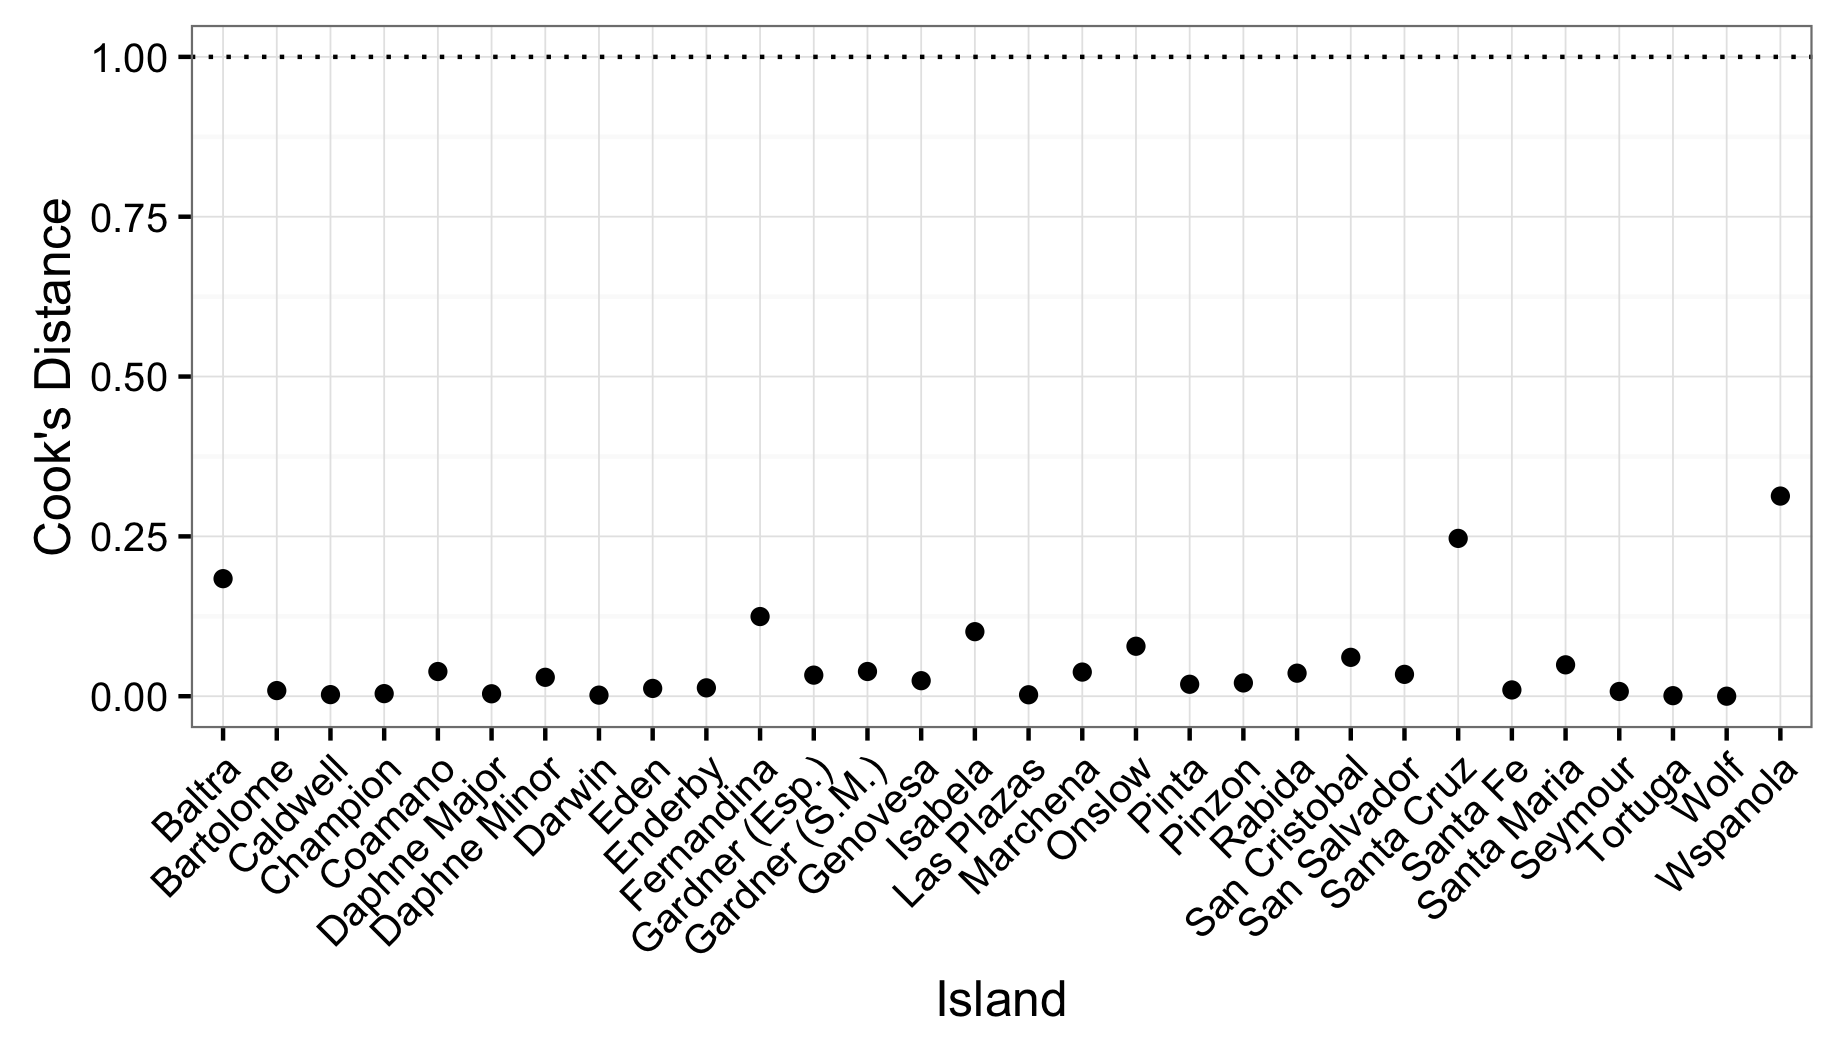
\includegraphics[width=4.25in]{2a_cd.png}
	\caption{Cook's Distances for each observation in the regression of Native on LogArea, LogElev, LogDistNear, and LogDistSc.}
	\label{fig:2a_cd}
\end{figure}


\part \textit{Nonnative Species}

A multiple regression of Nonnative on LogArea, LogElev, LogDistNear, LogDistSc, and LogAreaNear is shown below.

\begin{codeSmall}
> lmNonnative <- lm(formula = Nonnative ~ LogArea + LogElev +
+                     LogDistNear + LogDistSc + LogAreaNear,
+                   data = galapDataTransf)
> summary(lmNonnative)$coefficients
              Estimate Std. Error    t value  Pr(>|t|)
(Intercept)  90.078403 106.215060  0.8480756 0.4047749
LogArea      23.169532   6.700079  3.4580983 0.0020433
LogElev      -3.250762  20.849500 -0.1559156 0.8774036
LogDistNear -11.513117   7.437653 -1.5479502 0.1347209
LogDistSc    -7.436224   7.667156 -0.9698803 0.3417798
LogAreaNear  -7.974738   2.978570 -2.6773716 0.0131716
\end{codeSmall}$

After accounting for the relationship between Nonnative and Area (where we use the log-transformed value of Area, here), there is convincing evidence that the area of the nearest island (LogAreaNear) is associated with the number of nonnative species on the given island (two sided p-value = 0.0132 for a test that the LogAreaNear coefficient is zero). As compared to the regression of Native, there is no longer any evidence that the distance to the nearest island (LogDistNear) is associated with the number of nonnative species on the given island. None of the other variables have a significant relationship with the number of nonnative species.

Examining Cook's Distances for this model in Figure \ref{fig:2b_cd}, none of the observations are influential.

\begin{figure}[!h]
	\centering
	\captionsetup{width=0.8\textwidth}
	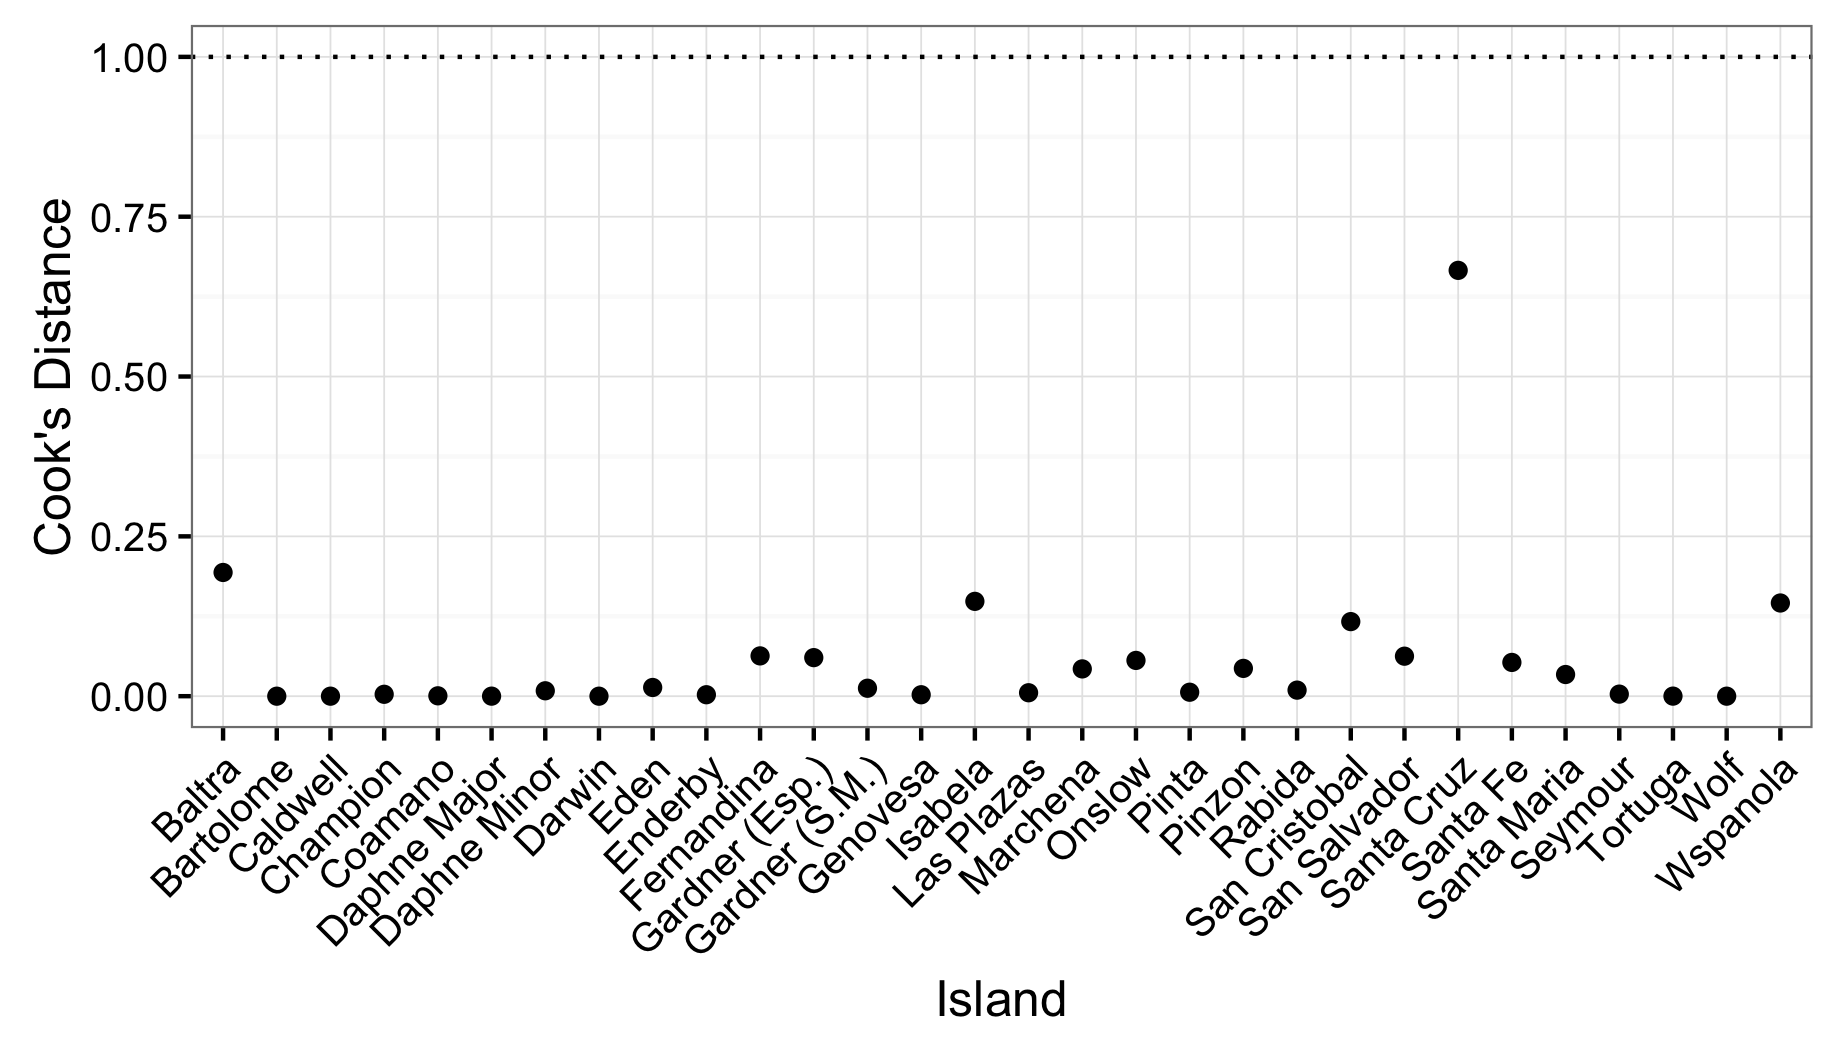
\includegraphics[width=4.25in]{2b_cd.png}
	\caption{Cook's Distances for each observation in the regression of Nonnative on LogArea, LogElev, LogDistNear, and LogDistSc.}
	\label{fig:2b_cd}
\end{figure}


\end{parts}




\titledquestion{\ramsey 20.11}
\setlength{\parindent}{1em}

\textit{The data in Display 20.14 are the launch temperatures (degrees Fahrenheit) and an indicator of O-ring failures for 24 space shuttle launches prior to the space shuttle Challenger disaster of January 28, 1986.}

\begin{parts}
\setlength{\parindent}{1em}


\part \textit{Fit the logistic regression of Failure (1 for failure) on Temperature. Report the estimated coefficients and their standard errors.}

The coefficients and associated standard errors for the logistic regression of Failure on Temperature are shown below.

\begin{codeSmall}
> glmShuttle <- glm(formula = Failure ~ Temperature,
+                   data = shuttleData, family = binomial)
> summary(glmShuttle)$coefficients
              Estimate Std. Error   z value   Pr(>|z|)
(Intercept) 10.8753491 5.70291251  1.906982 0.05652297
Temperature -0.1713205 0.08343865 -2.053251 0.04004824
\end{codeSmall}$



\part \textit{Test whether the coefficient of Temperature is 0, using Wald’s test. Report a one-sided p-value (the alternative hypothesis is that the coefficient is negative; odds of failure decrease with increasing temperature).}

Using Wald's test (confirming the Z statistic and associated two-sided p-value from part (a)), the data provides moderate evidence that the odds of failure decrease with increasing temperature (one-sided p-value  $0.0200$ from Wald's test).

\begin{codeSmall}
> tempEst <- (summary(glmShuttle)$coefficients)["Temperature", "Estimate"]
> tempSe <- (summary(glmShuttle)$coefficients)["Temperature", "Std. Error"]
> tempZstat <- (tempEst - 0)/tempSe
> tempPval <- pnorm(q = -1 * abs(tempZstat), mean = 0, sd = 1) ; tempPval # one-sided
[1] 0.02002412
\end{codeSmall}



\part \textit{Test whether the coefficient of Temperature is 0, using the drop-in-deviance test.}

Using the drop-in-deviance test (likelihood ratio test), the data provides moderate evidence that the odds of failure decrease with increasing temperature (one-sided p-value $0.0148$ from a drop-in-deviance test).

\begin{codeSmall}
> # fit a reduced model
> glmShuttleReduced <- glm(formula = Failure ~ 1,
+                   data = shuttleData, family = binomial)
> 
> # calculate the likelihood ratio test statistic and associated pvalue
> lrtStat <- summary(glmShuttleReduced)$deviance - summary(glmShuttle)$deviance
> lrtDf <- summary(glmShuttleReduced)$df[2] - summary(glmShuttle)$df[2]
> lrtPval <- pchisq(q = lrtStat, df = lrtDf, lower.tail = FALSE); lrtPval
[1] 0.01476632
> 
> # verify lrtPval using anova function
> anova(glmShuttle, glmShuttleReduced, test="LRT")
Analysis of Deviance Table

Model 1: Failure ~ Temperature
Model 2: Failure ~ 1
  Resid. Df Resid. Dev Df Deviance Pr(>Chi)  
1        22     23.030                       
2        23     28.975 -1  -5.9441  0.01477 *
---
Signif. codes:  0 ‘***’ 0.001 ‘**’ 0.01 ‘*’ 0.05 ‘.’ 0.1 ‘ ’ 1
\end{codeSmall}


\part \textit{Give a 95\% confidence interval for the coefficient of Temperature.}

A 95\% confidence interval for the coefficient of Temperature ($-0.1713$) is from $-0.3340$ to $-0.0078$.

\begin{codeSmall}
> tempEst
[1] -0.1713205
> tempEst + c(-1, 1) * (qnorm(p = 0.975, mean = 0, sd = 1) * tempSe)
[1] -0.334857256 -0.007783746
\end{codeSmall}


\part \textit{What is the estimated logit of failure probability at 31 degrees F (the launch temperature on January 28, 1986)? What is the estimated probability of failure?}

The estimated logit of failure probability at Temperature=31 is given by

\begin{align*}
\text{logit}(\pi) &= 10.8753 + (-0.1713) \times \text{Temperature} \\
&= 10.8753 + (-0.1713) \times 31 \\
&= 5.5647.
\end{align*}

\begin{codeSmall}
> logitPi <- predict(glmShuttle, data.frame(Temperature=31)) ; logitPi
       1 
5.564414 
\end{codeSmall}

The estimated probability of failure is given by

$$\pi = \frac{\exp(\text{logit}(\pi))}{1 + \exp(\text{logit}(\pi))} = \frac{\exp(5.5647)}{1 + \exp(5.5647)} = 0.9962.$$

\begin{codeSmall}
> exp(logitPi) / (1 + exp(logitPi))
        1 
0.9961828 
\end{codeSmall}


\part \textit{Why must the answer to part (e) be treated cautiously?}

The probability of failure at Temperature=31 must be treated cautiously, since the temperature at which we're making the prediction lays outside  the range of the Temperature variable values used to create the model, which range from 53 to 81 degrees F. This extrapolation is dangerous, since the model from part (a) isn't necessarily valid over a temperature outside of this range.

\end{parts}


\titledquestion{\ramsey 20.15}
\setlength{\parindent}{1em}

\textit{A study examined the association between nesting locations of the Northern Spotted Owl and availability of mature forests. Wildlife biologists identified 30 nest sites. The researchers selected 30 other sites at random coordinates in the same forest. On the basis of aerial photographs, the percentage of mature forest (older than 80 years) was measured in various rings around each of the 60 sites, as shown in Display 20.16.}

\begin{parts}
\setlength{\parindent}{1em}

\part \textit{Apply two-sample t-tools to these data to see whether the percentage of mature forest is larger at nest sites than at random sites.}

A boxplot of the percentage of mature forest around Nest sites and Random sites is shown in Figure \ref{fig:4a}. The distributions are nearly normal and have similar variances, making the two-sample t-test a good tool for this dataset\footnote{Note here that I've used \textit{all} of the measurements around the Nest and Random sites, not just those at PctRing1. The two-sample t-test gives the same conclusion when we restrict the dataset just to the PctRing1 measurements.}.

\begin{figure}[!h]
	\centering
	\captionsetup{width=0.8\textwidth}
	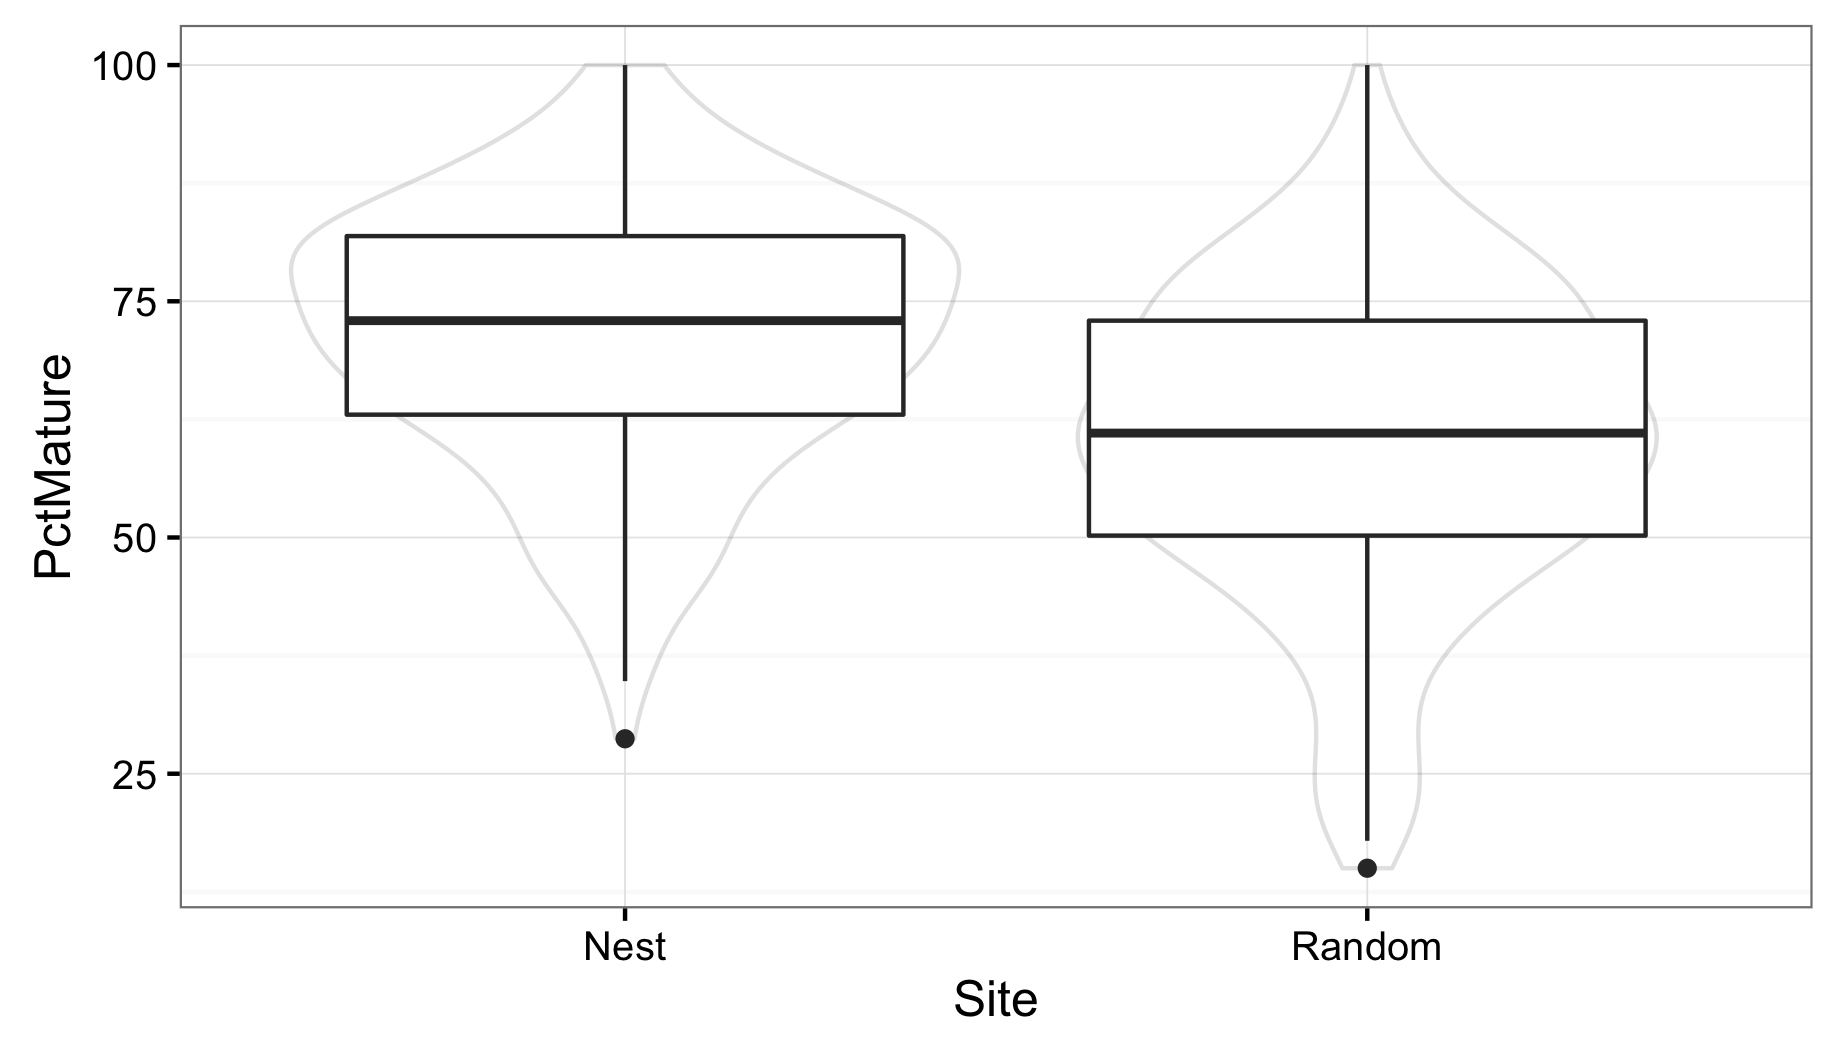
\includegraphics[width=4.25in]{4a.png}
	\caption{Boxplot of the percentage of mature forest around Nest sites and Random sites.}
	\label{fig:4a}
\end{figure}

\begin{codeSmall}
> tt <- t.test(formula=PctMature~Site, data=owlData2,
+              var.equal=TRUE, conf.level=0.95)
> diff(tt$estimate)[[1]] * -1
[1] 11.44524
> tt$p.value / 2
[1] 1.115927e-13
> tt$conf.int
[1]  8.477749 14.412727
attr(,"conf.level")
[1] 0.95
\end{codeSmall}$

The data provides overwhelming evidence that the mean percentage of mature forest is larger around nest sites than at random sites (one-sided p-value $1.1159 \time 10^{-13}$ from a two-sample t-test). The mean percentage of mature forest around Nest sites is $11.445$ percentage points higher than around Random sites (95\% confidence interval from $8.4777$ to $14.4127$ percentage points).


\part \textit{Construct a binary response variable that indicates whether a site is a nest site. Use logistic regression to investigate how large an area about the site has importance in distinguishing nest sites from random sites on the basis of mature forest.}

Boxplots of the percentage of mature forest around Nest sites and Random sites, for each ring radius is shown in Figure \ref{fig:4b_boxplots}.

\begin{figure}[!h]
	\centering
	\captionsetup{width=0.8\textwidth}
	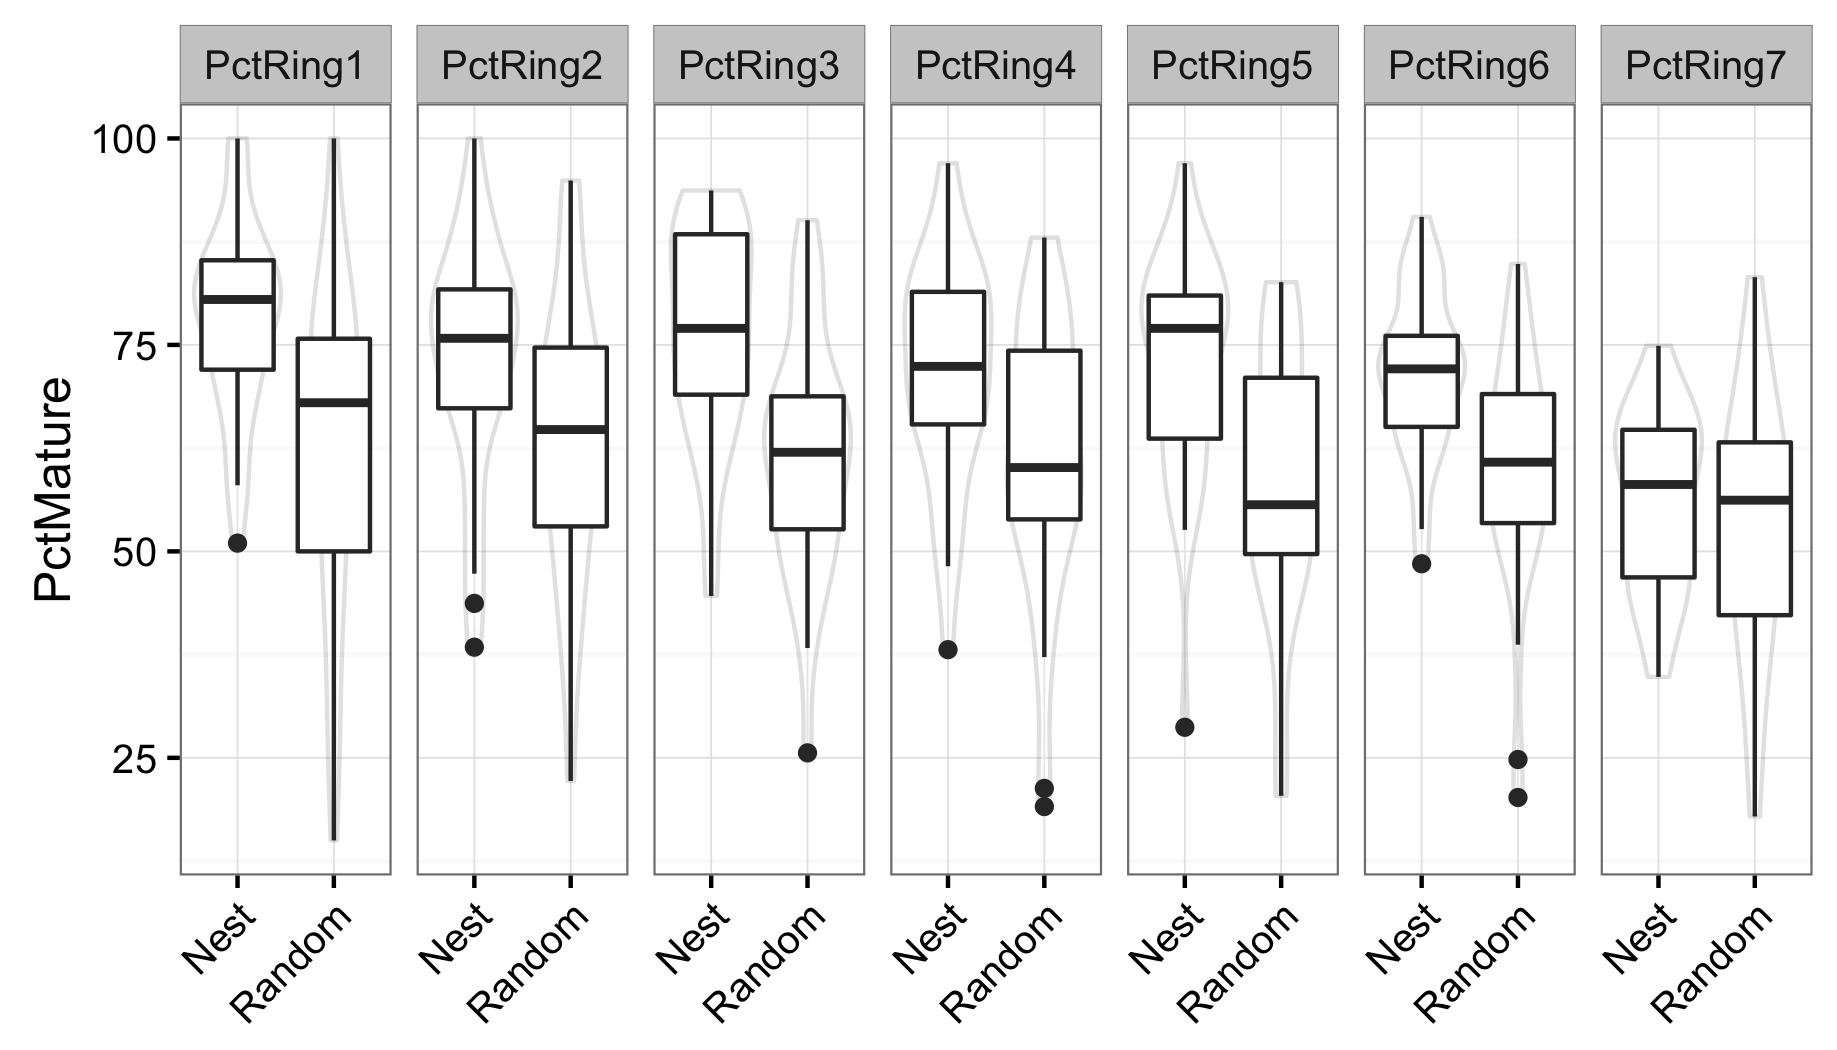
\includegraphics[width=4.25in]{4b_boxplots.png}
	\caption{Boxplots of the percentage of mature forest around Nest sites and Random sites, for each ring radius.}
	\label{fig:4b_boxplots}
\end{figure}

The binary response variable ``Nest'' indicates if a Site is a nest site (1) or a random site (0).

To investigate how large an area about the site has importance in distinguishing nest sites from random sites, we can fit a full model using the measurements at all 7 rings, and then using a drop-in-deviance test, compare it to a model with the innermost 6 rings, then to the model with the innermost 5 rings, etc., until finding the smallest model in which the p-value (from the drop-in-deviance test) is not significant.

A subset of the model definitions are shown below.

\begin{codeSmall}
# fit the 7 possible logistic regression models
glm7 <- glm(formula = Nest ~ .,
            data = select(owlData, Nest, PctRing1:PctRing7),
            family = binomial)
glm6 <- glm(formula = Nest ~ .,
            data = select(owlData, Nest, PctRing1:PctRing6),
            family = binomial)
...
glm1 <- glm(formula = Nest ~ .,
            data = select(owlData, Nest, PctRing1:PctRing1),
            family = binomial)
\end{codeSmall}

We then perform a drop-in-deviance test (likelihood ratio test), comparing the model with all 7 ring radii, \texttt{glm7}, to the model with only the innermost 6 ring radii, \texttt{glm6}.
\begin{codeSmall}
> anova(glm7, glm6, test="LRT")$"Pr(>Chi)"[[2]]
[1] 0.1335806
\end{codeSmall}$
The large p-value indicates that measurements at PctRing7 are not important in distinguishing nest sites from random sites.

Nest, we perform a drop-in-deviance test, comparing \texttt{glm7} to \texttt{glm5}.
\begin{codeSmall}
> anova(glm7, glm5, test="LRT")$"Pr(>Chi)"[[2]]
[1] 0.1496591
\end{codeSmall}$
The large p-value here indicates that measurements at PctRing7 and PctRing6 are not important in distinguishing nest sites from random sites.

Nest, we perform a drop-in-deviance test, comparing \texttt{glm7} to \texttt{glm4}.
\begin{codeSmall}
> anova(glm7, glm4, test="LRT")$"Pr(>Chi)"[[2]]
[1] 0.05645491
\end{codeSmall}$
The p-value of $0.0565$ is now significant (and much smaller than the first two tests), indicating that measurements at PctRing1 through PctRing5 \textit{are} important in distinguishing nest sites from random sites, and that measurements at PctRing6 and PctRing7 are not important.

We therefore use the model that includes PctRing1 through PctRing5.
\begin{codeSmall}
> summary(glm5)$coefficients
               Estimate Std. Error    z value   Pr(>|z|)
(Intercept) -8.35204928 2.48519484 -3.3607221 0.00077739
PctRing1     0.06293323 0.03385943  1.8586617 0.06307510
PctRing2    -0.11121477 0.04850913 -2.2926563 0.02186780
PctRing3     0.11739702 0.04711212  2.4918649 0.01270744
PctRing4    -0.01266591 0.03894926 -0.3251899 0.74503737
PctRing5     0.06359722 0.03519530  1.8069805 0.07076531
\end{codeSmall}$


\end{parts}


\titledquestion{} % Problem 5
\setlength{\parindent}{1em}




\titledquestion{} % Problem 6
\setlength{\parindent}{1em}




\end{questions}

%\listoftodos

\end{document}